\documentclass{standalone}
\usepackage{tikz}
\usetikzlibrary{shapes.geometric,patterns}
\usepackage{xcolor}

% Define colors
\definecolor{mainRed}{RGB}{255, 102, 102}
\definecolor{mainBlue}{RGB}{0, 0, 255}

\begin{document}
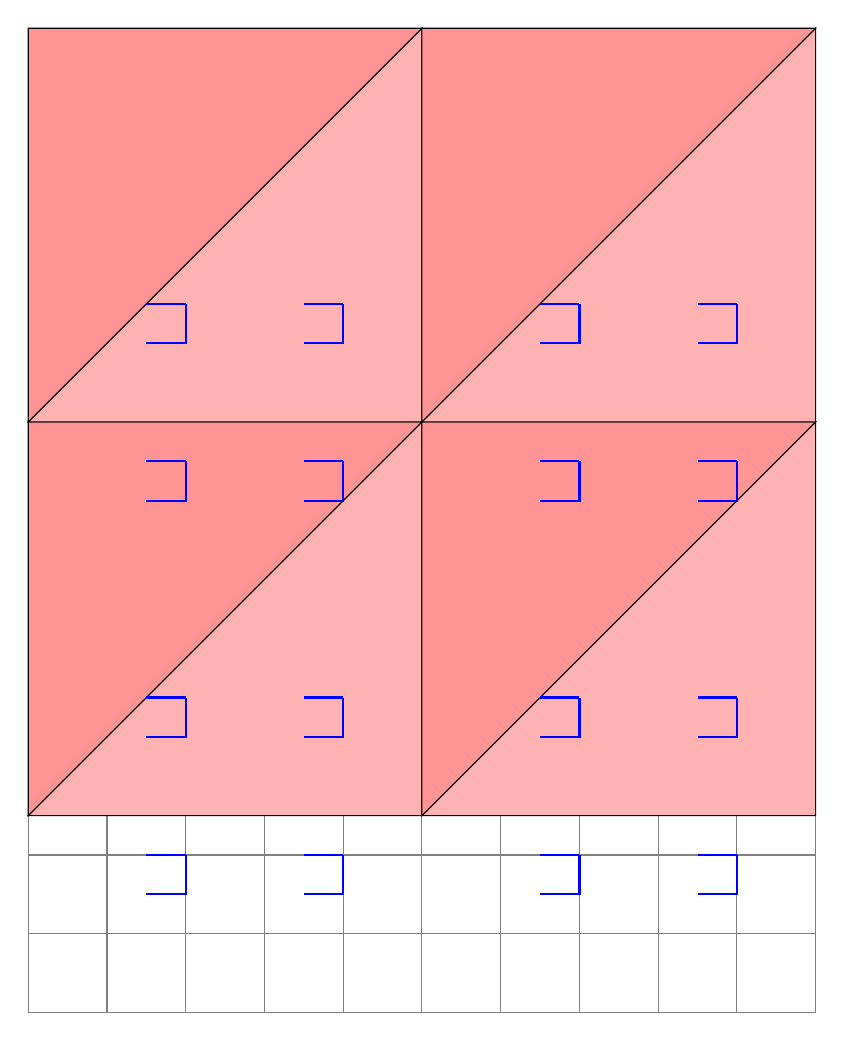
\begin{tikzpicture}
  % Background grid
  \draw[help lines, thin] (-5,-5) grid (5,5);

  % Red triangular patterns
  \foreach \x in {-5,0} {
    \foreach \y in {-2.5,2.5} {
      \fill[mainRed!50, draw=black, thin] (\x,\y) -- (\x+5,\y+5) -- (\x+5,\y) -- cycle;
      \fill[mainRed!70, draw=black, thin] (\x,\y) -- (\x+5,\y+5) -- (\x,\y+5) -- cycle;
    }
  }

  % Blue arrow-like patterns
  \foreach \x in {-3.5, -1.5, 1.5, 3.5} {
    \foreach \y in {-3.5, -1.5, 1.5, 3.5} {
      \draw[mainBlue, thick] (\x,\y) -- ++(0.5,0) -- ++(0,0.5);
      \draw[mainBlue, thick] (\x+0.5,\y) -- ++(0,0.5);
      \draw[mainBlue, thick] (\x,\y+0.5) -- ++(0.5,0);
    }
  }

  % Adjust coordinates for symmetry
  \foreach \x in {-3.5, -1.5, 1.5, 3.5} {
    \foreach \y in {-3.5, -1.5, 1.5, 3.5} {
      \draw[mainBlue, thick] (\x,\y) -- ++(0.5,0) -- ++(0,0.5);
      \draw[mainBlue, thick] (\x+0.5,\y) -- ++(0,0.5);
      \draw[mainBlue, thick] (\x,\y+0.5) -- ++(0.5,0);
    }
  }

\end{tikzpicture}
\end{document}